\chapter{Introducci\'on}

\label{Chapter1}

\section{Elecciones en Argentina}

En Argentina se celebran elecciones cada 2 a\~{n}os a excepci\'on de las presidenciales que se realizan cada 4
a\~{n}os. En Argentina se realizan tres tipos de elecciones:

\begin{itemize}
    \item Elecciones nacionales, para elegir a las autoridades federales del país: el Poder Ejecutivo, constituido por el
          Presidente y el vicepresidente y el Congreso Nacional, formado por Senadores y Diputados.
    \item Elecciones provinciales y de la Ciudad de Buenos Aires o locales, para elegir a las autoridades de cada provincia: los
          poderes ejecutivos de las provincias y sus legislaturas.
    \item Elecciones municipales, regidas por las leyes y procedimientos de cada provincia.
\end{itemize}

Si bien emitir el sufragio es diferente en cada una de ellas, generalmente consta de ingresar a un cuarto oscuro,
elegir el candidato que se desea y depositar el voto en una urna. Al finalizar la jornada, las autoridades de mesas
recuentan los votos y llenan una planilla a mano alzada donde se resume la cantidad de votos obtenidos por cada
candidato o partido pol\'itico. Dicha planilla es escaneada y enviada a traves de un telegrama correo argentino al
centro de c\'omputo para su procesamiento. Una vez all\'i, se contabilizan en un sistema inform\'atico una por una. Por
la metodolog\'ia de contabilizac\'ion, idealmente lo escrito a mano en el telegrama y lo computado en el sistema es lo
mismo. Sin embargo, como esta tarea es realizada por personas, es plausible pensar que pueden haber errores y demoras
en dicho proceso.

(TODO: ver de agregar un diagrama del proceso)

A su vez, durante la jornada electoral existe una ansiedad generalizada de la poblaci\'on por saber los resultados
parciales y finales de la misma, por lo que se debe contratar a una gran cantidad personas destinadas al centro de
c\'omputo. En las elecciones legislativas del 2021 se gastaron unos \$17.000 millones de pesos de los cuales \$4.000
millones de pesos fueron destinados a sueldos para el personal\footnote{Fuente:
    \href{https://www.cronista.com/economia-politica/Elecciones-legislativas-2021-cuanto-mas-se-gastara-por-el-coronavirus-segun-el-Presupuesto-20201004-0006.html}{El
        cronista}}. Mejorar el proceso manual de contabilizaci\'on de los telegramas supondr\'a un ahorro considerable en el
presupuesto de las elecciones, agilizar\'a la obtenci\'on de los resultados y aportar\'a transparencia al proceso en
general.

La presente tesis enfocar\'a el estudio en las elecciones legislativas de la provincia de Santa Fe del a\~{n}o 2021.
Los telegramas son p\'ublicos y se encuentran subidos en la
\href{https://op.elecciones.gob.ar/telegramas/generales2021/}{p\'agina oficial del estado argentino}. En el anexo
\ref{anexo:telegramas} se adjunta un ejemplo de uno de ellos.

\section{Digitalizaci\'on de telegramas electorales}

Una soluci\'on para bajar los costos de las elecciones podr\'ia ser la digitalizaci\'on autom\'atica de los telegramas
al sistema de c\'omputo general. Se puede entrenar un modelo de clasificaci\'on de d\'igitos y utilizarlo al momento de
la contabilizaci\'on de los votos.

La clasificaci\'on de d\'igitos es un problema resuelto desde \citeyear{lecun1998gradient}. En uno de los primeros
exponentes de lo que luego se denomin\'o {\it deep learning}, \cite{lecun1998gradient} se crea un nuevo dataset de
d\'igitos modificando el existente NIST y se propone la red neuronal LeNet-5 para la clasificaci\'on de los mismos. El
dataset MNIST consiste de 60.000 imagenes de entrenamiento y 10.000 de testing. Cada una de las im\'agenes es de un
tama\~{n}o de 28x28 pixeles.

\begin{figure}[ht]
    \centering
    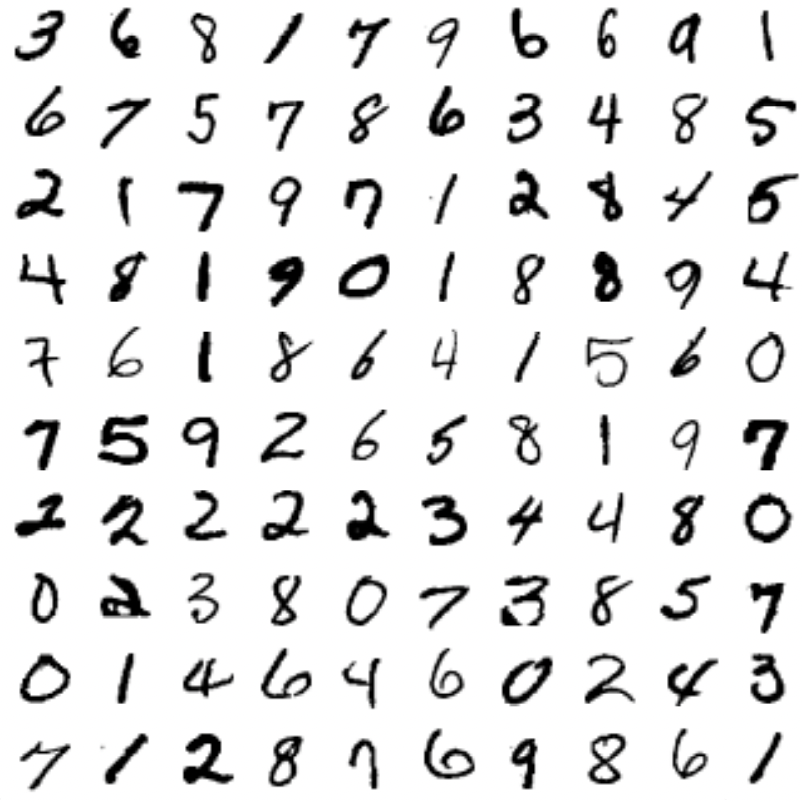
\includegraphics[width=0.6\textwidth]{chapter1/mnist.png}
    \caption{Ejemplos del dataset MNIST}
    \label{fig:mnist}
\end{figure}

La red posee capas convolucionales las cuales se encargan de extraer caracter\'isticas o patrones de las im\'agenes
para luego ser procesadas por capas densas que se encargan de la clasificaci\'on.

\begin{figure}[ht]
    \centering
    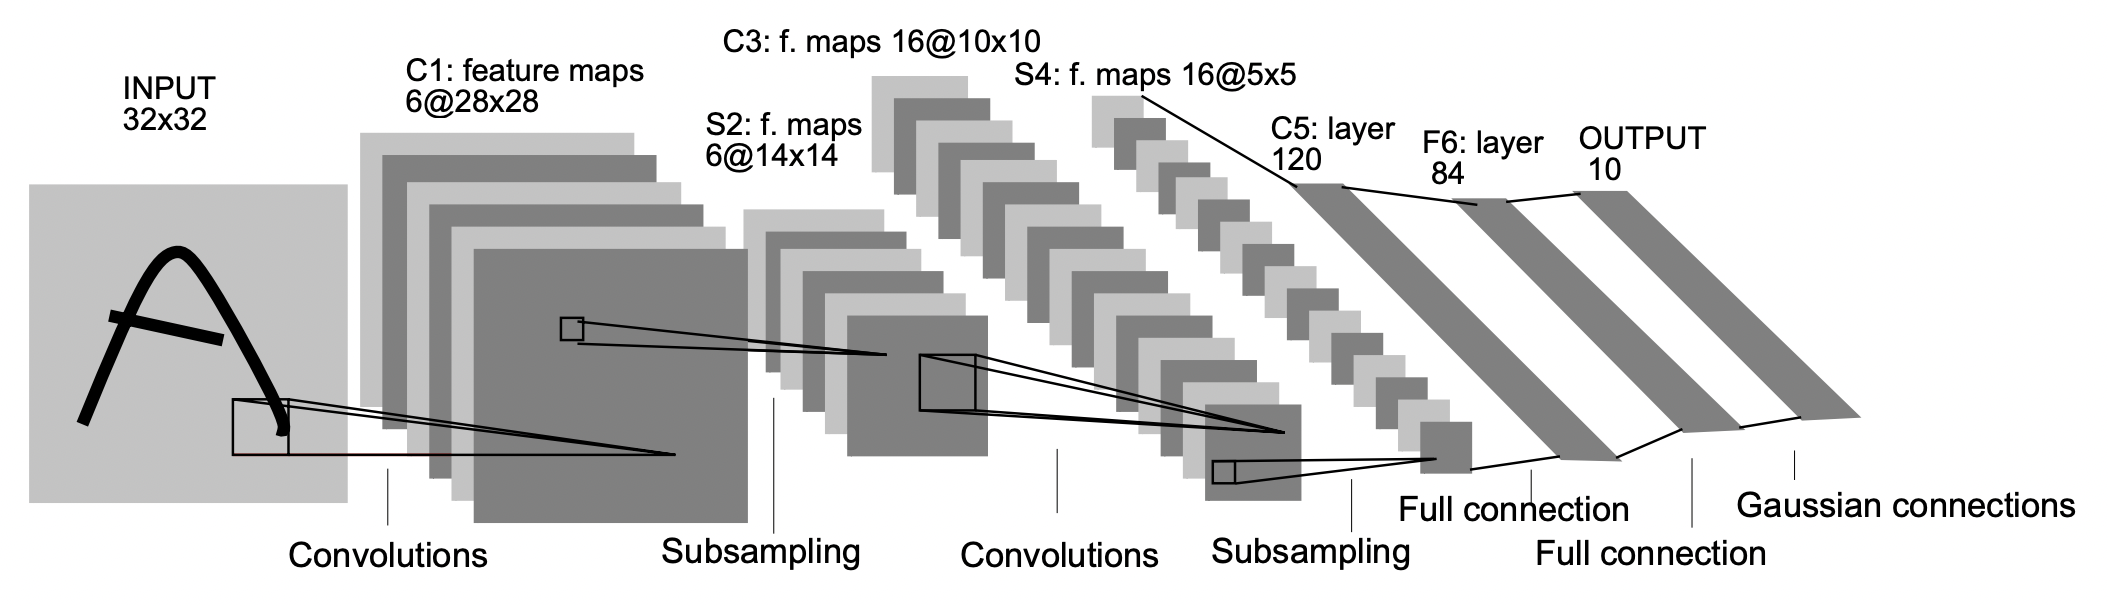
\includegraphics[width=1\textwidth]{chapter1/lenet5.png}
    \caption{Arquitectura de la red LeNet-5}
    \label{fig:lenet-5}
\end{figure}

Sin embargo, aunque LeNet-5 (o cualquier otro modelo) presente buenas m\'etricas de performance, no significa que pueda
ser aplicado a otro dataset de d\'igitos. El cuadro \ref{tab:lenet-distintos-datasets} muestra la precisi\'on que se
obtiene al entrenar una red LeNet-5 en distintos datasets de d\'igitos: MNIST \parencite{lecun1998gradient}, USPS \parencite{hull1994database} y SVHN \parencite{netzer2011reading}. La arquitectura de la red posee la capacidad de aprender los patrones de cada uno de los
ellos pero no logra generalizar a otros. Si bien cada uno de ellos muestran los mismos n\'umeros, lo hacen de forma
diferente. Esto se debe al {\it sesgo} que existe en los datos. Al entrenar un modelo, el mismo aprende a reconocer
caracter\'isticas propias del dataset que le permite resolver el problema, incluyendo el sesgo. \'Esto hace que un
problema "sencillo" de clasificaci\'on de im\'agenes de 28x28 pixeles no sea trivial. Todos los datasets se encuentran
sesgados de alguna forma y es imposible armarlos de tal forma que no presenten alg\'un nivel de sesgo \parencite{khosla2012undoing}. Cuando los datos con los que se quiere evaluar un modelo provienen de un dominio o
distribuci\'on diferente al de entrenamiento, se est\'a ante un {\it dataset shift} \parencite{quinonero2008dataset}. Es decir, se le muestra al modelo cosas que nunca vi\'o y, por lo tanto, no sabe
reconocer.

\begin{table}[ht]
    \centering
    \begin{tabular}{cccc}
        \toprule
        {}                                                & \multicolumn{3}{c}{Testing}                                                                                               \\
        {}                                                & MNIST                                             & USPS                              & SVHN                              \\
        Entrenamiento                                     & 
\includegraphics[width=16px]{chapter1/mnist3.png}
        
\includegraphics[width=16px]{chapter1/mnist6.png}
        
\includegraphics[width=16px]{chapter1/mnist8.png} & 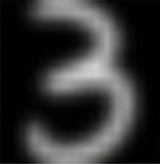
\includegraphics[width=16px]{chapter1/usps3.png}
        
\includegraphics[width=16px]{chapter1/usps6.png}
        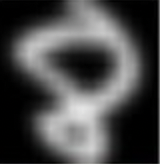
\includegraphics[width=16px]{chapter1/usps8.png}  & 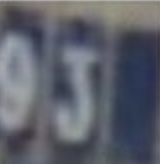
\includegraphics[width=16px]{chapter1/svhn3.png}
        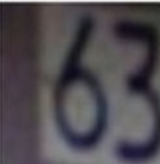
\includegraphics[width=16px]{chapter1/svhn6.png}
        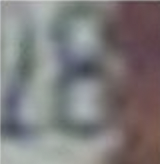
\includegraphics[width=16px]{chapter1/svhn8.png}                                                                                                                              \\
        \midrule
        MNIST                                             & \multirow{2}{*}{\textbf{99.17\%}}                 & \multirow{2}{*}{78.08\%}          & \multirow{2}{*}{31.50\%}          \\
        
\includegraphics[width=16px]{chapter1/mnist3.png}
        
\includegraphics[width=16px]{chapter1/mnist6.png}
        
\includegraphics[width=16px]{chapter1/mnist8.png} &                                                   &                                   &                                   \\
        USPS                                              & \multirow{2}{*}{57.10\%}                          & \multirow{2}{*}{\textbf{95.42\%}} & \multirow{2}{*}{26.94\%}          \\
        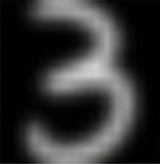
\includegraphics[width=16px]{chapter1/usps3.png}
        
\includegraphics[width=16px]{chapter1/usps6.png}
        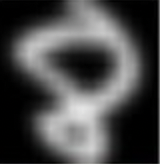
\includegraphics[width=16px]{chapter1/usps8.png}  &                                                   &                                   &                                   \\
        SVHN                                              & \multirow{2}{*}{61.92\%}                          & \multirow{2}{*}{64.28\%}          & \multirow{2}{*}{\textbf{89.52\%}} \\
        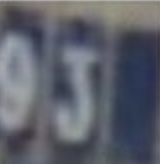
\includegraphics[width=16px]{chapter1/svhn3.png}
        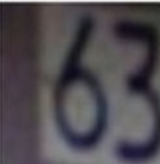
\includegraphics[width=16px]{chapter1/svhn6.png}
        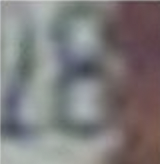
\includegraphics[width=16px]{chapter1/svhn8.png}  &                                                   &                                   &                                   \\
        \bottomrule
    \end{tabular}
    \caption{Precisi\'on obtenida al entrenar una LeNet-5 con distintos datasets de d\'igitos.}
    \label{tab:lenet-distintos-datasets}
\end{table}

El problema que abordar\'a la presente tesis es c\'omo se puede entrenar un modelo que aprenda a clasificar d\'igitos
para ser utilizados en los telegramas de elecciones legislativas de Santa Fe del 2021 (distinto al dominio de
entrenamiento) pese al sesgo existente en los datasets mencionados previamente. Para poder lograrlo, se necesita
entrenar de cierta manera un modelo en alguno de los datasets p\'ublicos etiquetados de forma tal que pueda generalizar
a otro similar.

\section{Transferencia de conocimiento}

Cuando se habla de {\it Deep learning}, se hace referencia a una serie de algoritmos de {\it machine learning} que son
capaces de utilizar m\'ultiples capas de procesamiento de forma que puedan aprender representaciones de los datos con
diferentes niveles de abstracci\'on \parencite{lecun2015deep}. Estos algoritmos, denominados redes neuronales profundas (o DNNs por sus siglas en ingl\'es),
poseen la capacidad de encontrar variables que expliquen la naturaleza del comportamiento de los datos.

Los modelos obtenidos a partir del {\it deep learning} han demostrado tener gran capacidad de aprendizaje para todo
tipo de problemas, como ser {\it computer vision} \parencite{szeliski2010computer, redmon2016yolo}, procesamiento del lenguaje natural \parencite{devlin2018bert}, reconocimiento del habla \parencite{hannun2014deep}, juegos \parencite{silver2016mastering}, generaci\'on de im\'agenes a partir de descripciones \parencite{ramesh2022dalle2}, entre otros.

Aunque la utilidad de estos modelos se encuentra demostrada y d\'ia a d\'ia son utilizados en diferentes \'ambitos de
la vida, presentan un gran problema: la enorme cantidad de datos etiquetados que requieren para su entrenamiento. La
mayor\'ia de los modelos que mejores m\'etricas de performance presentan, necesitan millones de datos en sus datasets
de entrenamiento. Esto implica que, para que los mismos sean de utilidad, resultan de suma importancia los procesos de
recolecci\'on y etiquetado de los datos. La eficacia de los modelos queda altamente relacionada con la calidad de los
datos que se posean o se logren conseguir. El etiquetado de los datos es una tarea costosa, ineficiente y hasta a veces
resulta inviable de realizar \parencite{reis2022data}. En el caso de las elecciones, no es posible tener de antemano la clasificaci\'on de los mismos,
ya que son completados a mano a\~{n}o a a\~{n}o por diferentes personas.

Una posible soluci\'on a este problema consiste en emular la capacidad que tienen los humanos de adquirir conocimiento
relevante en un \'area y aplicarlo en otra similar \parencite{thrun1998learning}. Es decir, poder {\it transferir} lo aprendido. En el caso del {\it deep learning}, lo que se
busca es que la red aprenda representaciones lo suficientemente generales para que despues sean utilizados en el
entrenamiento de una tarea similar. La idea es acortar los tiempos de entrenamiento, mejorar las predicciones y hacer
modelos m\'as robustos.
